\documentclass[../mathNotesPreamble]{subfiles}

\begin{document}
%  \relscale{1.4} %TODO
  \section{9.3: Answering Questions about the Mean of a Population}
    \begin{defn*}
      Suppose that we wish to estimate a population mean $\mu$ based on a sample mean $\overline{x}$.
      \begin{itemize}
        \item A \textbf{confidence interval} is an interval about the point estimate $\overline{x}$ that we can be confident contains the true population mean $\mu$:
          \[\overline{x}\pm m\]
        \item The \textbf{margin of error (ME)} is half the width of the confidence interval. When estimating a population proportion, the margin of error is
          \[m=t^* SE\]
          where 
          \[SE_{est}=\frac{s}{\sqrt{n}}\]
        \item The \textbf{confidence level} measures how often the estimation method is successful. A larger confidence level results in a larger margin of error.
      \end{itemize}
    \end{defn*}
    \vspace*{2\baselineskip}
    
    The multiplier $t^*$ is found using the $t$-distribution and $n-1$ degrees of freedom.
    \pagebreak
    
    The $t$-distribution is used when
    \begin{itemize}
      \item the sample size is small %(e.g. smaller than 25)
      \item the population standard deviation is unknown
    \end{itemize}
    As the sample size $n$ (and degrees of freedom, $n-1$) increases, the $t$-distribution gets closer to the Standard Normal Distribution. 
    
    The graph below shows the $t$-distribution in black where the degrees of freedom are $1$, $2$, $4$, and $30$, and the Standard Normal Distribution in blue.

    \begin{center}
      \begin{tikzpicture}[scale=1.0, declare function={
        N=50;
        mu=0; sig=1;
        xmin=mu-3.2*sig;
        xmax=mu+3.2*sig;
        ymin=-0.1*gauss(mu,mu,sig);
        h=0.08*gauss(mu,mu,sig);}]
        \begin{axis}[
          every axis plot post/.append style={
          mark=none, domain={-3.2:3.2},samples=N,smooth},
          axis line style={black,->},
          axis x line=middle,
%          ymin=ymin, ymax={1.1*gauss(mu,mu,sig)},
          axis y line=none,
          every axis x label/.style={at={(current axis.right of origin)},anchor=north},
          width=0.8\linewidth, height=1.1*\axisdefaultheight,
          ticklabel style={font=\footnotesize,inner sep=0.5pt,fill=white,opacity=1.0, text opacity=1},
          clip=false,
          ]
          %This plot needs to be compiled using 
          %"pdflatex --shell-escape" in order to utilize gnuplots
          \foreach \n in {1,2,4,30}{
%          \pgfplotsinvokeforeach {1,2,4,30}{
%            \def\n{#1} %explicitly define \n
            \addplot gnuplot [black,thick,smooth,no marks]{\students};
%              node [pos=0.5, anchor=west, xshift=3em] {$n=#1$};
            }
            \addplot[-, blue] expression[domain=-3.5:3.5] {gauss(x,0,1)};
        \end{axis}
      \end{tikzpicture}
    \end{center}
    \pagebreak
    
    \begin{center}
      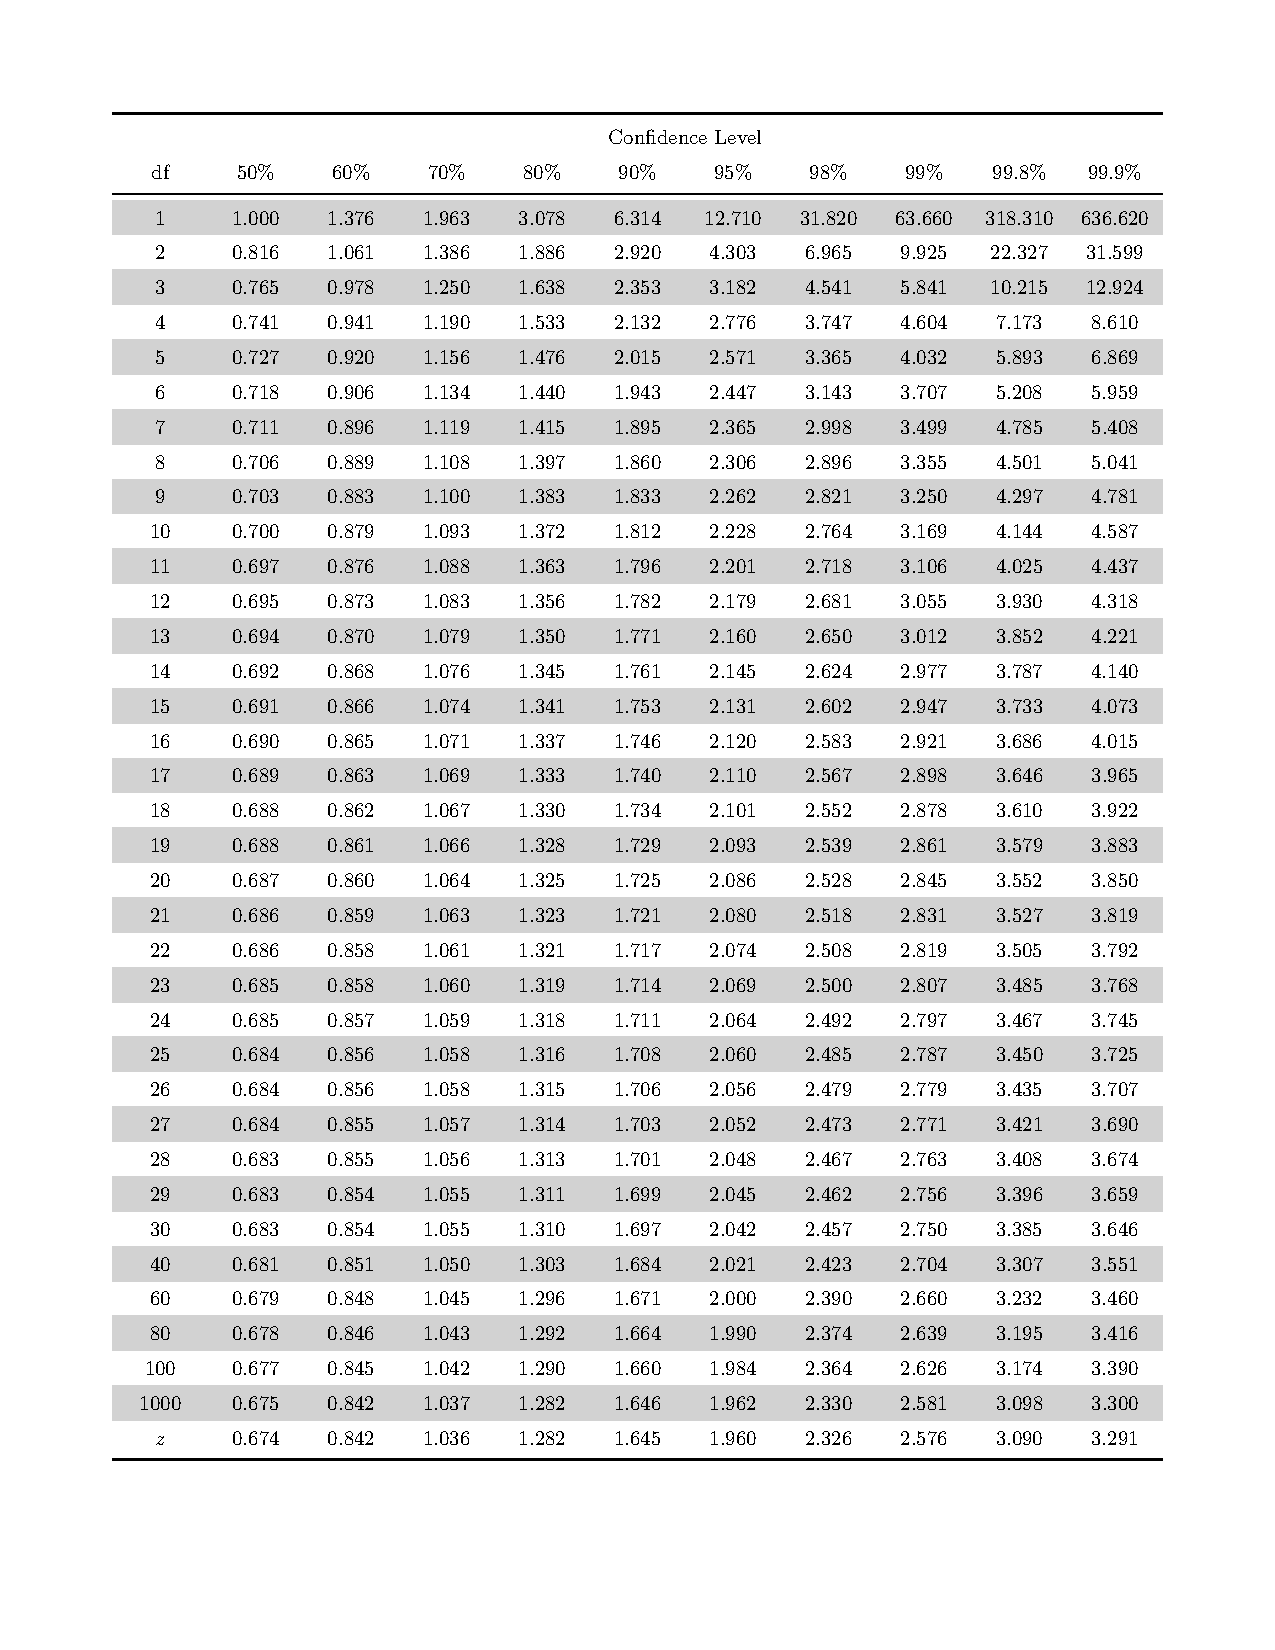
\includegraphics[width=0.925\linewidth]{t_score_table}
    \end{center}
    \pagebreak
    
    \begin{ex*}
      A random sample of 35 two-year colleges in 2014-2015 had a mean tuition of $\$4,173$, with a standard deviation of $\$2,590$. Find the 90\% and 95\% confidence intervals and interpret their results.
    \end{ex*}
    \vspace*{\stretch{1}}
    
    \begin{ex*}
      A study to test the life of iPad batteries reports that in a random sample of 30 iPads, the mean battery life was 9.7 hours, and the standard deviation was 1.2 hours. 
    \end{ex*}
    \begin{extasks}[after-item-skip=\stretch{1}](1)
      \task Compute a 95\% confidence interval and interpret the results. 
      \task Suppose Apple claims the iPad has a mean battery life of 10 hours. Based on this confidence interval, do we reject or fail to reject this claim?
    \end{extasks}
    \vspace*{\stretch{0.5}}
    \pagebreak

    \begin{ex*}
      Suppose I am interested in estimating my mean commute time. Over the course of a week, I record my commute times:
    \end{ex*}
    \begin{center}
      \begin{tabularx}{0.45\linewidth}{@{}*{5}{Y}@{}}\toprule
        18.96&
        20.65&
        17.47&
        19.38&
        17.11\\\bottomrule
      \end{tabularx}
    \end{center}
    Compute a 95\% confidence interval for my actual commute times.    
    
  \pagebreak
\end{document}
